% !TeX root = main.tex
\chapterimage{chapter-07-code-org.jpg}
\chapter{Code.org}\label{capitolo-7-code.org}
% Evita dilatazioni verticali fra testo e figure alte nel solo capitolo 7.
\raggedbottom

Dopo aver esplorato concetti fondamentali dell'Informatica (come gli \textbf{algoritmi} e la \textbf{rappresentazione delle informazioni}) e aver compreso come dare \textbf{istruzioni} a un \textbf{esecutore}, è il momento di passare alla \textbf{programmazione} vera e propria usando il computer o il tablet.

In questa sezione ti guideremo passo passo nell'utilizzo dei corsi proposti da Code.org, un'associazione non profit che da anni promuove l'accesso universale all'informatica, con risorse gratuite e attività pensate specificamente per bambini e bambine.

Per la scuola primaria, Code.org propone percorsi per insegnare la programmazione usando un linguaggio visuale a blocchi, cioè in cui le istruzioni sono blocchetti grafici da trascinare e collegare come pezzi di LEGO®.

Grazie a personaggi familiari (come Angry Birds, Plants vs Zombies, Frozen, Star Wars ecc.), l'attività risulta motivante e vicina all'immaginario di bambini e bambine. Le sfide proposte sono strutturate in modo progressivo (partono dall'imparare a trascinare i blocchi e progrediscono in maniera molto graduale) e forniscono un alto livello di scaffolding (supporto guidato). Ad ogni livello il sistema dà feedback immediato, suggerimenti e obiettivi chiari da raggiungere. Anche se può sembrare un approccio limitato in termini di creatività, questa modalità basata su puzzle è estremamente utile per i principianti, perché riduce la paura di sbagliare e accompagna passo dopo passo nella scoperta dei concetti fondamentali. I bambini e le bambine imparano così ad apprezzare gli errori come parte del processo (\textbf{debugging}) e a sviluppare strategie di problem solving in un contesto giocoso e controllato.

\section{Traguardi e obiettivi generali }\label{traguardi-e-obiettivi-generali-4}

\begin{itemize}
\item
  Orientarsi nell'ambiente di programmazione Code.org Studio (interfaccia, comandi base, esecuzione e reset del programma).
\item
  Creare programmi in sequenza, disponendo le istruzioni in un ordine logico per muovere un personaggio sullo schermo.
\item
  Riconoscere il ruolo della ripetizione per eseguire più volte una stessa istruzione o sequenza di istruzioni in modo efficiente.
\item
  Creare disegni e percorsi geometrici, sviluppando precisione nell'uso delle sequenze e delle ripetizioni e collegando la programmazione ai concetti spaziali.
\item
  Sperimentare la strategia di prova ed errore, interpretando i feedback dell'ambiente per correggere gli errori (debugging).
\end{itemize}

\section{Prerequisiti }\label{prerequisiti-4}

Le attività di questo capitolo risultano più efficaci se studenti e studentesse hanno già avuto qualche esperienza di base con i concetti informatici introdotti nei capitoli precedenti. In particolare è consigliabile, ma non obbligatorio, che abbiano lavorato sui movimenti su griglia (Capitolo~\ref{capitolo-4-movimenti-su-una-griglia}).

Dal punto di vista strumentale, avere un po' di dimestichezza con il mouse o il touch (cliccare, trascinare, rilasciare) è un vantaggio. Tuttavia, i primi livelli dei corsi (in particolare il Corso A) sono pensati proprio per esercitare queste abilità di base: se per alcuni è la prima esperienza al computer o tablet, Code.org può diventare un'ottima occasione guidata per imparare a usare il mouse o il touch mentre si lavora sui concetti informatici.

\section{Preparazione }\label{preparazione-7}

\subsection{Programma il Futuro }\label{programma-il-futuro}

In Italia, le attività di Code.org sono state diffuse grazie al progetto del Laboratorio CINI Informatica e Scuola, patrocinato dal MIM, chiamato \emph{Programma il Futuro} (PiF).

Il progetto fornisce da oltre 11 anni un ampio supporto agli insegnanti italiani nell'introduzione dell'Informatica nella scuola. Ti consigliamo di visitare il sito \urloriginale{https://programmailfuturo.it/}.

\subsection{Iscrizione dell'insegnante e della classe a Code.org }\label{iscrizione-dellinsegnante-e-della-classe-a-code.org}


Il modo più semplice per iscriversi a Code.org è seguire le istruzioni sul sito di \emph{Programma il Futuro}: \linkbreve{pifIscrizione}. In questo modo ti iscriverai contemporaneamente sia a PiF sia a Code.org.


Una volta completato questo passo, confermando la registrazione a \emph{Programma il Futuro} cliccando sul link presente nella mail ricevuta all'indirizzo e-mail usato per la registrazione, è possibile accedere a Code Studio (\linkbreve{codeorgIscrizione}) usando lo stesso indirizzo e-mail e la stessa password.

Successivamente si può procedere con la creazione di una classe. Per creare una classe, bisogna accedere alla sezione Controllo (che è comunque la pagina predefinita al login su \urloriginale{https://studio.code.org}), dedicata alla gestione delle classi esistenti e alla creazione di nuove. Si può indicare anche il livello della classe e il corso seguito (scelte non obbligatorie, ma consigliate per agevolare studenti e studentesse).

\begin{attenzione}
  Anche se Code.org tende a suggerire corsi più nuovi, al momento (\meseannocorrente) quelli tradotti con cura in italiano e verificati sono quelli del \textbf{2021}. Non hai bisogno di passare ai corsi più recenti.

  Da qui in poi, quando ci riferiamo ai Corsi di Code.org intendiamo sempre la versione del 2021 in italiano.
\end{attenzione}

Suggeriamo di compiere le seguenti scelte:

\begin{itemize}
\item
  Tipi di login → Immagine password.
\item
  Nome della classe → attribuire un nome significativo.
\item
  Grado → indicare la classe (es. 3 per la terza primaria).
\item
  Assegna curriculum → Fondamenti di informatica - Corso A - Versione 2021 (o il corso da cui vuoi partire: vedi più avanti).
\item
  Impostazioni avanzate:

  \begin{itemize}
  \item
    Esercizi Supplementari (Lesson Extras) → Sì
  \item
    Programmazione in coppia → Sì. Abilitare questa opzione consente agli studenti di lavorare in due o più sullo stesso dispositivo, mantenendo aggiornati i progressi dei profili di tutti.
  \end{itemize}
\end{itemize}


Salvando queste informazioni (che possono comunque essere tutte successivamente modificate), la classe viene identificata da un codice di 6 caratteri, ad esempio ABCDEF.

Una volta creata la classe, devono essere aggiunti studenti e studentesse. L'unica informazione obbligatoria è un nome/nickname univoco per ciascuno. Consigliamo di non inserire dati personali (es. usare un numero e/o un nomignolo). Una volta che la classe sarà completa\footnote{Potrebbe capitare che venga richiesto di accettare le condizioni relative alla privacy e all'uso dei cookie.}, si potrà consegnare a ciascuno un foglio autogenerato con le istruzioni e la relativa immagine-password per accedere alla classe.

Assicurati che tutti abbiate il testo visualizzato in italiano. Se così non fosse, scorri la pagina fino in fondo e seleziona ``Italiano'' dal menu a tendina delle lingue.

Dalla sezione Controllo, puoi monitorare le tue classi e i progressi di studenti e studentesse.

\subsection{Accesso di studenti e studentesse a Code.org }\label{accesso-di-studenti-e-studentesse-a-code.org}

Tutte le lezioni al computer o sul tablet iniziano con gli studenti e le studentesse che effettuano l'accesso alla classe su Code.org, raggiungendo il sito \urloriginale{https://studio.code.org}, inserendo il codice della classe (es. ABCDEF) nella parte destra (``Inserisci il codice di 6 lettere della tua classe'') e poi premendo su ``Go''.


\subsection{E se non voglio creare nessun account?}


Puoi accedere direttamente ai corsi, ma ovviamente i progressi non verranno salvati e non sarà possibile creare una classe.


\begin{itemize}
  \item Link diretto alle attività interattive del Corso A: \linkbreve{codeA}
  \item Link diretto alle attività interattive del Corso B: \linkbreve{codeB}
  \item Link diretto alle attività interattive del Corso C: \linkbreve{codeC}
\end{itemize}


\section{Attività 1: introduzione a Code.org}

\ruoliattivita{\ruoloProgrammatore}

I corsi di ``Introduzione all'Informatica'' di Code.org forniscono ambienti molto guidati; una volta entrati, studenti e studentesse impareranno velocemente a muoversi all'interno di essi.

Specialmente per chi non ha dimestichezza con l'uso del mouse (o, meno probabile, del tablet) per trascinare i blocchi, ti consigliamo di iniziare dal Corso A (2021).

Come insegnante, puoi guardare qui la panoramica sulle lezioni del Corso A: \linkbreve{codeAguida}


Nota, ad esempio, che:

\begin{itemize}
\item
  Alcune lezioni (1, 3, 7, 11) sono unplugged (contraddistinte dal pulsante ``Attività tradizionale'')
\item
  Per ogni lezione, puoi

  \begin{itemize}
  \item
    leggere il piano di lavoro di ciascuna lezione: contiene una panoramica, traguardi, obiettivi, consigli per lo svolgimento, una pianificazione precisa di ogni fase della lezione;
  \item
    decidere se mostrarla o nasconderla ai tuoi studenti.
  \end{itemize}
\end{itemize}


La Lezione 2 (la prima lezione ``tecnologica'') aiuta a prendere confidenza con il trascinamento dei blocchi.

La Lezione 4 (seconda lezione ``tecnologica'') è la prima in cui ci si trova nell'ambiente del ``labirinto''. Ci sono dei livelli da superare, come in un normale videogioco, ma studenti e studentesse dovranno programmare un personaggio affinché raggiunga i suoi obiettivi. Fai loro sperimentare alcuni livelli (almeno fino al Livello 4 compreso) e, nel frattempo, comincia a far osservare loro le varie componenti dell'interfaccia che si trovano davanti.

Alcune lezioni iniziano con un breve video che presenta l'ambiente o un nuovo concetto. Guardalo prima della lezione e controlla la lingua dell'audio o dei sottotitoli, poi valuta se mostrarlo a tutta la classe oppure rivederlo quando emerge una difficoltà. Per esempio, il \hrefbreve{codeVideo}{primo livello della Lezione 4 del Corso A (2021)} (\linkbreve{codeVideo}) propone il video \emph{Introduzione a Code Studio}, con sottotitoli italiani.

Ipotizziamo che tu abbia davanti il livello 6 della Lezione 4 del corso A (2021), di cui non possiamo riprodurre lo screenshot per copyright.
Puoi trovarlo al link: \linkbreve{codeEs}

Prima di presentare le spiegazioni che seguono, puoi proporre una breve esplorazione a coppie: ``Osservate la schermata, provate i pulsanti e scoprite a che cosa servono le sue diverse parti. Disegnate sul quaderno uno schema dello schermo e completatelo con nomi e brevi spiegazioni''. Chiedi di distinguere dove si legge la consegna, dove si osserva il personaggio, dove si trovano i blocchi disponibili e dove si costruisce il programma. Ogni coppia può poi confrontare le proprie scoperte con quelle delle altre.

\begingroup
\setlength{\tabcolsep}{7pt}
\setlength{\arrayrulewidth}{0.4pt}
\arrayrulecolor{black!40}
\renewcommand{\arraystretch}{1.15}
\setlength{\LTleft}{0pt}
\setlength{\LTright}{0pt}
\newcommand{\figurainterfacciacodeorg}[2]{%
  \centering\vspace{5pt}%
  \includegraphics[#2]{img/codeorg-interfaccia/#1.png}\par\vspace{5pt}%
}
\begin{longtable}{|>{\raggedright\arraybackslash}m{\dimexpr0.40\linewidth-2\tabcolsep-1.5\arrayrulewidth\relax}|>{\raggedright\arraybackslash}m{\dimexpr0.60\linewidth-2\tabcolsep-1.5\arrayrulewidth\relax}|}
\hline
\rowcolor{black!12}
\textbf{Interfaccia} & \textbf{Spiegazione} \\
\hline
\endfirsthead
\hline
\rowcolor{black!12}
\textbf{Interfaccia} & \textbf{Spiegazione} \\
\hline
\endhead
\figurainterfacciacodeorg{area-gioco}{width=\linewidth}\label{credito:codeorg-interfaccia-gioco-1}
& \textbf{Area di gioco} è la parte in cui si vedono i personaggi e gli effetti dell'esecuzione \\
\hline
\figurainterfacciacodeorg{istruzioni}{width=\linewidth}\label{credito:codeorg-interfaccia-istruzioni-1}
& \textbf{Istruzioni} descrive invece il compito da svolgere per superare il livello. I pulsanti per l'accessibilità permettono di vedere la consegna con font più grande, e anche di ascoltarla. L’ascolto della consegna può essere utile anche a chi sta ancora imparando a leggere.  \\
\hline
\figurainterfacciacodeorg{blocchi}{height=5.2cm}\label{credito:codeorg-interfaccia-blocchi-1}
& \textbf{Blocchi}: sono le istruzioni che il computer capisce e che alunne e alunni possono usare (anche più volte) per indicare al personaggio cosa fare per raggiungere l'obiettivo. Nelle attività unplugged dei capitoli precedenti abbiamo chiamato questo elenco Manuale delle istruzioni. \\
\hline
\figurainterfacciacodeorg{area-lavoro}{width=\linewidth}\label{credito:codeorg-interfaccia-lavoro-1}
& \textbf{Area di lavoro}: qui c'è il programma, cioè la sequenza di istruzioni che alunne e alunni vogliono dare al personaggio. I blocchi devono essere attaccati tra loro come mattoncini LEGO®.

Il primo numero indica il numero di blocchi attualmente usati (cioè quelli presenti nell'area di lavoro). Il secondo numero indica una quantità di blocchi sufficiente per risolvere il livello; non sempre è il minimo possibile.
Infatti, in alcuni casi, il numero di blocchi necessari per risolvere il puzzle è inferiore a quello indicato come sufficiente\footnote{Un esempio può chiarire: la scritta “3/10” indica 3 blocchi usati e 10 indicati come sufficienti per risolvere l'esercizio. A volte, il livello potrebbe essere risolvibile anche con meno blocchi, per esempio 8: in tal caso, il numero di blocchi necessari è inferiore a quello indicato come sufficiente.}. \\
\hline
\figurainterfacciacodeorg{esegui}{width=2.7cm}\label{credito:codeorg-interfaccia-pulsanti-1}
& \textbf{Pulsante Esegui}: alunne e alunni possono premerlo per eseguire il programma nell'area di lavoro e vedere l'effetto che fa nell'area di gioco! \\
\hline
\figurainterfacciacodeorg{fai-un-passo}{width=3.7cm}\label{credito:codeorg-interfaccia-pulsanti-2}
& \textbf{Pulsante ``Fai un passo''}: alunne e alunni possono premerlo per eseguire il programma nell'area di lavoro un'istruzione alla volta. Possono usarlo se il personaggio non fa quello che si aspettano! \\
\hline
\figurainterfacciacodeorg{livelli}{width=\linewidth}\label{credito:codeorg-interfaccia-livelli-1}
& \textbf{I livelli di questa lezione}: quando i pallini saranno tutti verdi, alunne e alunni possono passare alla prossima lezione. \\
\hline
\end{longtable}
\endgroup


\subsubsection{E il corso B?}

Queste considerazioni valgono ugualmente anche per il Corso B (2021). \linkbreve{codeBguida}

Il Corso B è allineato al Corso A, ma si distingue per attività unplugged più approfondite e una selezione più varia di esercizi al computer\footnote{\linkbreve{pifCorsi} \linkbreve{pifCorsoA} \linkbreve{pifCorsoB}}.

\section{Attività 2: Labirinti (corsi A e B)}

\ruoliattivita{\ruoloProgrammatore}

Le lezioni 4, 5, 6, 8, 9 del Corso A e 3, 4, 5, 7, 8 del Corso B sono tutte collocate nell'ambiente ``Labirinti''.

In questo tipo di livelli, ci sarà un personaggio (spesso dei videogiochi o dei film conosciuti) che si muove su una griglia/scacchiera (analogamente a quanto già visto nel Capitolo~\ref{capitolo-4-movimenti-su-una-griglia}) e deve

\begin{itemize}
\item
  raggiungere altri personaggi (spesso nemici);
\item
  raccogliere oggetti.
\end{itemize}

Chi programma deve immaginare di guardare la scena dall'alto e quindi potrà indicare al personaggio come muoversi seguendo i punti cardinali (Nord, Sud, Ovest, Est) per raggiungere il suo obiettivo. Si tratta quindi di movimenti descritti rispetto a un sistema di riferimento assoluto.

Ecco una guida sintetica sull'effetto dei blocchi che i bambini possono incontrare nei livelli del Labirinto:

\begingroup
\manualeimpostazioni
\setlength{\LTleft}{0pt}
\setlength{\LTright}{0pt}
\arrayrulecolor{guideManualeBordo}
\begin{longtable}{|K{\dimexpr0.50\linewidth-2\tabcolsep-1.5\arrayrulewidth\relax}|J{\dimexpr0.50\linewidth-2\tabcolsep-1.5\arrayrulewidth\relax}|}
\hline
\manualetitolo{2}{LABIRINTI A E B}
\manualeintestazione
\endfirsthead
\endhead
\multicolumn{2}{r@{}}{\small\itshape continua\ldots} \\
\endfoot
\endlastfoot
\manualeimmagini{
\includegraphics[scale=0.9]{img/codeorg-svg-cap07/pdf/codeorg-blocco-n.pdf}\label{credito:codeorg-labirinto-direzioni-1}} & Il personaggio si muove in alto (verso Nord) di una casella. \\
\hline
\manualeimmagini{
\includegraphics[scale=0.9]{img/codeorg-svg-cap07/pdf/codeorg-blocco-s.pdf}\label{credito:codeorg-labirinto-direzioni-2}} & Il personaggio si muove in basso (verso Sud) di una casella. \\
\hline
\manualeimmagini{
\includegraphics[scale=0.9]{img/codeorg-svg-cap07/pdf/codeorg-blocco-e.pdf}\label{credito:codeorg-labirinto-direzioni-3}} & Il personaggio si muove a destra (verso Est) di una casella. \\
\hline
\manualeimmagini{
\includegraphics[scale=0.9]{img/codeorg-svg-cap07/pdf/codeorg-blocco-o.pdf}\label{credito:codeorg-labirinto-direzioni-4}} & Il personaggio si muove a sinistra (verso Ovest) di una casella. \\
\hline
\manualeimmagini{
\includegraphics[scale=0.9]{img/codeorg-raccolta/pdf/codeorg-prendi-gemma.pdf}\label{credito:codeorg-prendi-gemma-1}\hspace{6pt}%

\includegraphics[scale=0.9]{img/codeorg-raccolta/pdf/codeorg-prendi-pannocchia.pdf}\label{credito:codeorg-prendi-pannocchia-1}}
& Se si trova su una casella che contiene l'oggetto raffigurato, il personaggio ne raccoglie uno. \\
\hline
\manualeimmagini{
\includegraphics[scale=0.9]{img/codeorg-ripeti-manuale/pdf/codeorg-ripeti.pdf}\label{credito:codeorg-ripeti-manuale-1}}
& Le istruzioni inserite al suo interno vengono eseguite il numero di volte scelto dal menu a tendina. \\
\hline
\end{longtable}
\manualeripristinacolore
\endgroup

\subsubsection{Ripeti}

\ruoliattivita{\ruoloProgrammatore\quad\ruoloEsecutore}

Per evitare di usare tante volte lo stesso blocco, è possibile usare il blocco \textbf{ripeti}.
Nell'esempio qui sotto a sinistra, il programma ripete 3 volte l'istruzione ``spostati di una casella verso Nord''; in quello a destra vengono ripetute 3 volte, nell'ordine, le due istruzioni ``verso Nord'' e poi ``verso Est''.

\begin{center}
\raisebox{-0.5\height}{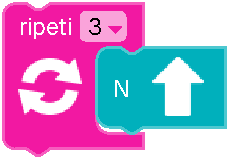
\includegraphics[scale=0.9]{img/codeorg-svg-cap07/pdf/codeorg-ripeti3n.pdf}\label{credito:codeorg-labirinto-ripetizioni-1}}\hspace{3em}\raisebox{-0.5\height}{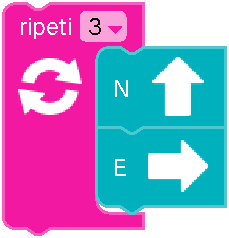
\includegraphics[scale=0.9]{img/codeorg-svg-cap07/pdf/codeorg-ripeti3ne.pdf}\label{credito:codeorg-labirinto-ripetizioni-2}}
\end{center}

\ruoliattivita{\ruoloEsecutore}

Per controllare che il blocco \textbf{ripeti} sia stato compreso, mostra uno alla volta i due programmi appena presentati e proponi questa consegna: ``Riscrivi il programma senza usare Ripeti. Quali istruzioni verranno eseguite, e in quale ordine? Disegna sul quaderno il percorso a partire da una casella che hai scelto''. In questa fase alunne e alunni assumono il ruolo di esecutori: devono interpretare un programma già scritto.


Chiedi di formulare la risposta prima della prova al computer, poi confrontatela con la figura seguente. Nel secondo caso si ripete tre volte l'intera sequenza di due istruzioni: Nord, Est, Nord, Est, Nord, Est.

\begin{center}
\begin{minipage}{0.94\linewidth}
\centering
\begin{minipage}[t]{0.47\linewidth}
\centering\vspace{0pt}
\textbf{Una sola istruzione ripetuta tre volte}\par\smallskip
\begin{tabular}{@{}c@{\hspace{0.4em}}c@{\hspace{0.4em}}c@{}}
\raisebox{-0.5\height}{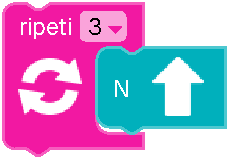
\includegraphics[scale=0.9]{img/codeorg-svg-cap07/pdf/codeorg-bozza-ripeti3n.pdf}\label{credito:codeorg-labirinto-ripetizioni-3}} &
$\Longleftrightarrow$ &
\raisebox{-0.5\height}{
\includegraphics[scale=0.9]{img/codeorg-svg-cap07/pdf/codeorg-bozza-sequenza3n.pdf}\label{credito:codeorg-labirinto-sequenze-1}}
\end{tabular}
\end{minipage}\hfill
\begin{minipage}[t]{0.47\linewidth}
\centering\vspace{0pt}
\textbf{Una sequenza di due istruzioni ripetuta tre volte}\par\smallskip
\begin{tabular}{@{}c@{\hspace{0.4em}}c@{\hspace{0.4em}}c@{}}
\raisebox{-0.5\height}{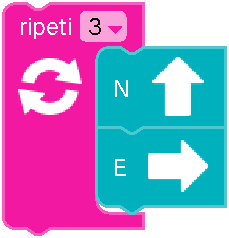
\includegraphics[scale=0.9]{img/codeorg-svg-cap07/pdf/codeorg-bozza-ripeti3ne.pdf}\label{credito:codeorg-labirinto-ripetizioni-4}} &
$\Longleftrightarrow$ &
\raisebox{-0.5\height}{
\includegraphics[scale=0.9]{img/codeorg-svg-cap07/pdf/codeorg-bozza-sequenza3ne.pdf}\label{credito:codeorg-labirinto-sequenze-2}}
\end{tabular}
\end{minipage}
\end{minipage}
\end{center}


\section{Attività 3: Artista (corsi A e B)}

\ruoliattivita{\ruoloProgrammatore}

La Lezione 10 del Corso A e la Lezione 9 del Corso B si svolgono nell'ambiente dell'Artista.

In questo tipo di livelli, si controlla un artista che, muovendosi sul foglio (esprimendo i movimenti sempre rispetto a un sistema di riferimento assoluto con i punti cardinali), potrà realizzare disegni geometrici.

La tabella seguente mostra l'effetto dei blocchi che alunni e alunne possono incontrare. Le direzioni restano sempre le stesse rispetto al foglio.

\begingroup
\manualeimpostazioni
\setlength{\LTleft}{0pt}
\setlength{\LTright}{0pt}
\arrayrulecolor{guideManualeBordo}
\begin{longtable}{|K{\dimexpr0.50\linewidth-2\tabcolsep-1.5\arrayrulewidth\relax}|J{\dimexpr0.50\linewidth-2\tabcolsep-1.5\arrayrulewidth\relax}|}
\hline
\manualetitolo{2}{ARTISTA A E B}
\manualeintestazione
\endfirsthead
\endhead
\multicolumn{2}{r@{}}{\small\itshape continua\ldots} \\
\endfoot
\endlastfoot
\manualeimmagini{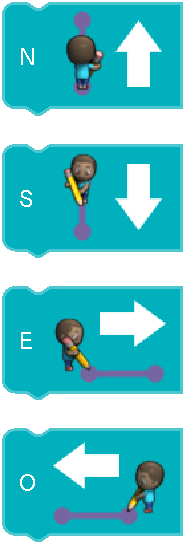
\includegraphics[scale=0.8]{img/codeorg-svg-cap07/pdf/codeorg-artista-nseo.pdf}\label{credito:codeorg-artista-direzioni-1}\hspace{6pt}%
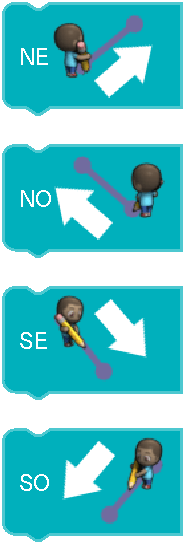
\includegraphics[scale=0.8]{img/codeorg-svg-cap07/pdf/codeorg-artista-diagonali.pdf}\label{credito:codeorg-artista-direzioni-2}}
& L'artista si muove e disegna un segmento nella direzione indicata, anche in diagonale.\par\medskip
\begin{center}
\begin{tikzpicture}[x=0.9cm,y=0.9cm,font=\sffamily\scriptsize]
  \draw[gray!50] (0,0) circle (0.8);
  \foreach \a in {0,45,...,315} \draw[line width=1.1pt,ocre,-stealth] (0,0) -- (\a:1.3);
  \node[font=\sffamily\scriptsize\bfseries] at (0,1.8) {NORD (N)};
  \node[font=\sffamily\scriptsize\bfseries] at (0,-1.8) {SUD (S)};
  \node[font=\sffamily\scriptsize\bfseries,anchor=west] at (1.5,0) {EST (E)};
  \node[font=\sffamily\scriptsize\bfseries,anchor=east] at (-1.5,0) {OVEST (O)};
  \node[anchor=south west,align=center] at (1.05,1.05) {NORD-EST\\(NE)};
  \node[anchor=south east,align=center] at (-1.05,1.05) {NORD-OVEST\\(NO)};
  \node[anchor=north east,align=center] at (-1.05,-1.05) {SUD-OVEST\\(SO)};
  \node[anchor=north west,align=center] at (1.05,-1.05) {SUD-EST\\(SE)};
\end{tikzpicture}
\end{center} \\
\hline
\manualeimmagini{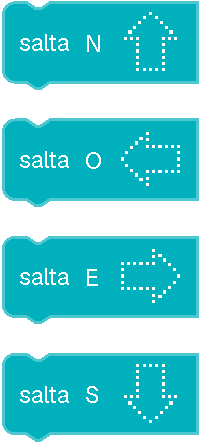
\includegraphics[scale=0.8]{img/codeorg-artista-cap07/pdf/codeorg-salta-cardinali.pdf}\label{credito:codeorg-artista-salti-1}\hspace{6pt}%
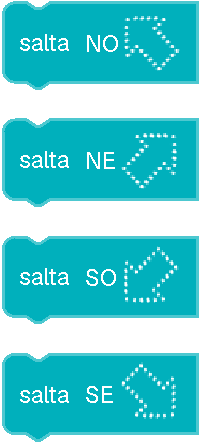
\includegraphics[scale=0.8]{img/codeorg-svg-cap07/pdf/codeorg-salta.pdf}\label{credito:codeorg-artista-salti-2}}
& L’artista si muove come nei blocchi sopra,
ma senza lasciare traccia. \\
\hline
\manualeimmagini{
\includegraphics[width=0.96\linewidth]{img/codeorg-artista-cap07/pdf/codeorg-imposta-schema.pdf}\label{credito:codeorg-artista-schema-1}\par\smallskip
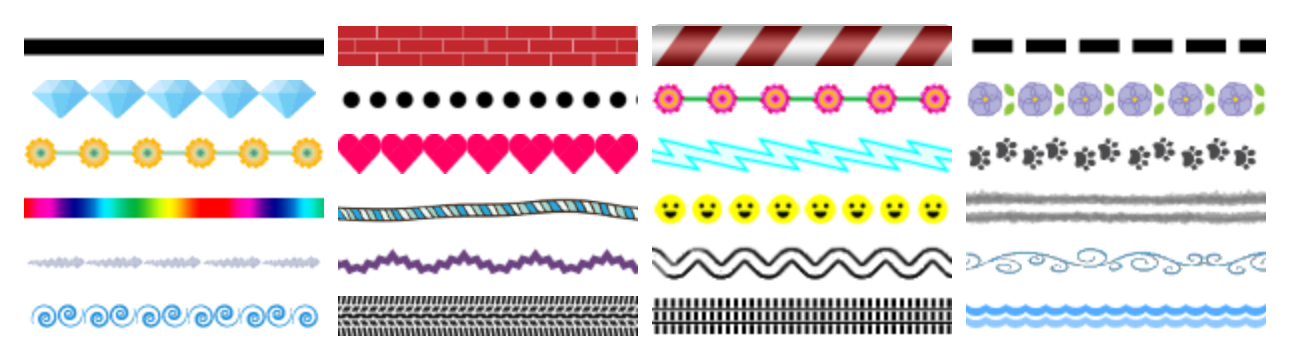
\includegraphics[width=0.96\linewidth]{img/codeorg-artista-schermate/schema-menu.png}\label{credito:codeorg-artista-menu-schema-1}}
& Da questa istruzione in poi, l'artista disegna usando lo schema scelto fra quelli proposti. Il menu permette di scegliere la trama del tratto. \\
\hline
\manualeimmagini{
\includegraphics[scale=0.85]{img/codeorg-svg-cap07/pdf/codeorg-imposta-colore.pdf}\label{credito:codeorg-artista-colore-1}}
& Da questa istruzione in poi, l'artista disegna usando una penna del colore scelto. \\
\hline
\manualeimmagini{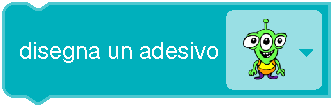
\includegraphics[scale=0.9]{img/codeorg-svg-cap07/pdf/codeorg-adesivo.pdf}\label{credito:codeorg-artista-adesivo-1}}
& L'artista stampa, nel punto in cui si trova, l'adesivo scelto, come un timbro. \\
\hline
\end{longtable}
\manualeripristinacolore
\endgroup

Si può cambiare la velocità con cui l'artista disegna: il disegno viene tracciato più lentamente quando il cursore è vicino alla tartaruga, più velocemente quando è vicino alla lepre. Rallentare l'esecuzione aiuta a osservare l'effetto di ogni istruzione.

\begin{center}
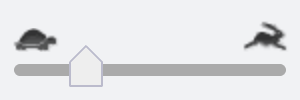
\includegraphics[width=5.5cm]{img/codeorg-artista-schermate/velocita.png}\label{credito:codeorg-artista-velocita-1}
\end{center}

\subsubsection{Leggere un programma e prevedere il disegno}

\ruoliattivita{\ruoloEsecutore}

Puoi proporre queste attività anche su un foglio quadrettato, senza computer o tablet. Mostra inizialmente soltanto il programma qui sotto, indica un punto di partenza e chiedi: ``Che cosa disegna l'artista se esegue queste istruzioni?''. Alunni e alunne assumono il ruolo di esecutori: leggono i blocchi dall'alto verso il basso e tracciano il percorso, mantenendo uguali i passi orizzontali e verticali.

Con il programma seguente, l'artista realizza una scaletta dall'alto in basso. Confronta il disegno ottenuto con la soluzione e, se possibile, fai verificare la previsione nell'ambiente Artista.

\begingroup
\setlength{\tabcolsep}{7pt}
\setlength{\arrayrulewidth}{0.4pt}
\arrayrulecolor{black!40}
\renewcommand{\arraystretch}{1.2}
\begin{center}
\begin{tabular}{|>{\centering\arraybackslash}m{\dimexpr0.50\linewidth-2\tabcolsep-1.5\arrayrulewidth\relax}|>{\centering\arraybackslash}m{\dimexpr0.50\linewidth-2\tabcolsep-1.5\arrayrulewidth\relax}|}
\hline
\rowcolor{black!12}
\sffamily\bfseries PROGRAMMA & \sffamily\bfseries SOLUZIONE \\
\hline
\vspace{5pt}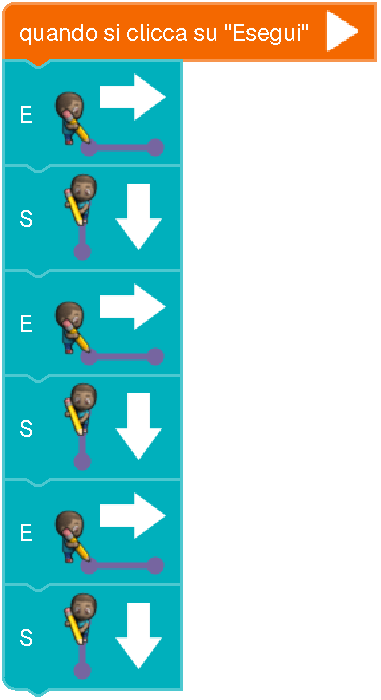
\includegraphics[scale=0.6]{img/codeorg-artista-cap07/pdf/codeorg-scala-programma.pdf}\label{credito:codeorg-artista-scaletta-programma-1}\par\vspace{5pt}
& \vspace{5pt}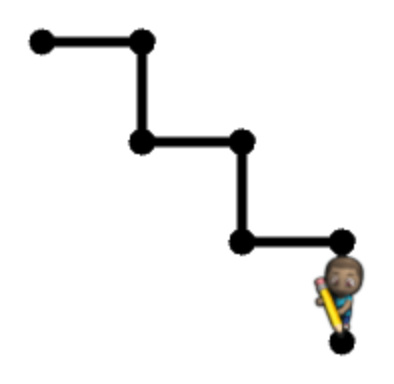
\includegraphics[width=0.85\linewidth]{img/codeorg-artista-schermate/scaletta.png}\label{credito:codeorg-artista-scaletta-disegno-1}\par\vspace{5pt} \\
\hline
\end{tabular}
\end{center}
\endgroup

\subsubsection{Scrivere un programma per un disegno}

Ora proponi il compito inverso (su carta o al computer): ``Aiuta l'artista a realizzare questi disegni''. Mostra soltanto i due disegni.

Di seguito sono riportate anche due possibili soluzioni.

\begin{center}
\begin{minipage}[t]{0.48\linewidth}
\centering\vspace{0pt}
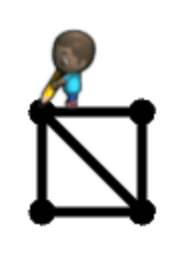
\includegraphics[height=3.3cm]{img/codeorg-artista-schermate/quadrato-diagonale.png}\label{credito:codeorg-artista-quadrato-diagonale-disegno-1}\par\medskip
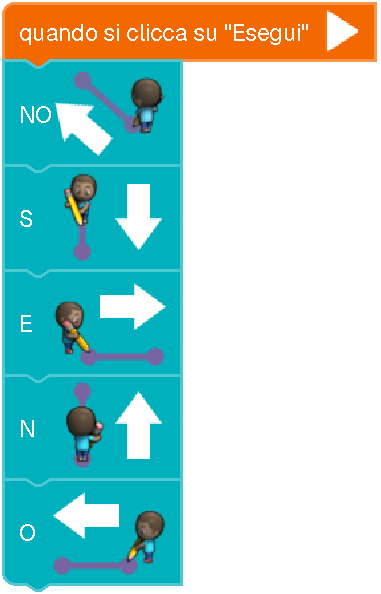
\includegraphics[scale=0.6]{img/codeorg-artista-cap07/pdf/codeorg-quadrato-diagonale-programma.pdf}\label{credito:codeorg-artista-quadrato-diagonale-programma-1}
\end{minipage}\hfill
\begin{minipage}[t]{0.48\linewidth}
\centering\vspace{0pt}
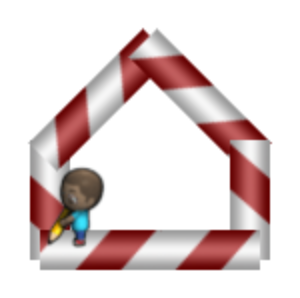
\includegraphics[height=3.3cm]{img/codeorg-artista-schermate/casa-strisce.png}\label{credito:codeorg-artista-casa-strisce-disegno-1}\par\medskip
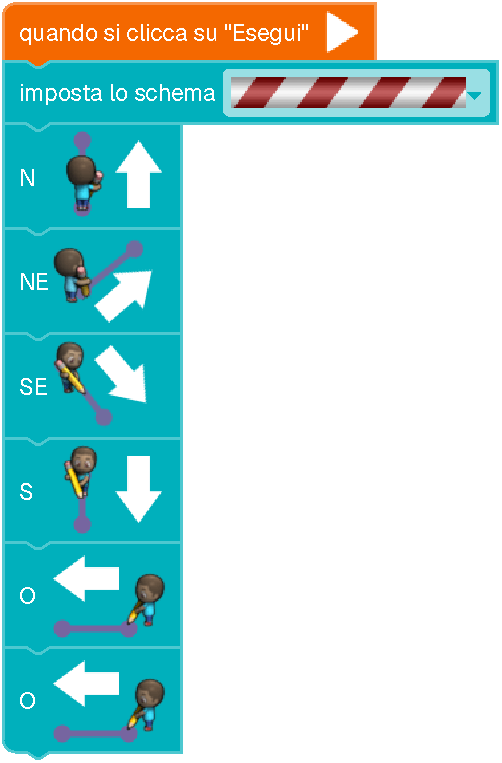
\includegraphics[scale=0.6]{img/codeorg-artista-cap07/pdf/codeorg-casa-schema-programma.pdf}\label{credito:codeorg-artista-casa-strisce-programma-1}
\end{minipage}
\end{center}

Per provare i programmi al computer, alunne e alunni possono usare il \textbf{Laboratorio Artista pre-scolare}: \linkbreve{artistaBase}. Qui alunni e alunne possono realizzare liberamente i propri disegni, senza un compito preassegnato.

Se qualcuno non sa cosa disegnare, ecco altri due suggerimenti che puoi dare loro (il secondo è più sfidante).

\begin{center}
\begin{minipage}[t]{0.48\linewidth}
\centering\vspace{0pt}
\parbox[c][3.2cm][c]{\linewidth}{\centering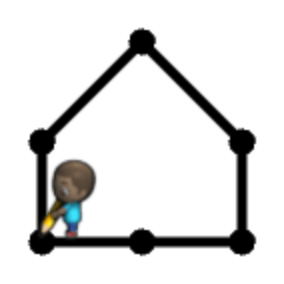
\includegraphics[height=3.2cm]{img/codeorg-artista-schermate/casa.png}\label{credito:codeorg-artista-casa-disegno-1}}\par\medskip
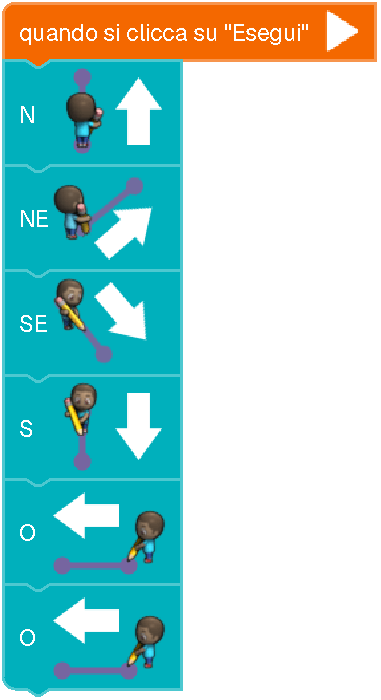
\includegraphics[scale=0.5]{img/codeorg-artista-cap07/pdf/codeorg-casa-programma.pdf}\label{credito:codeorg-artista-casa-programma-1}
\end{minipage}\hfill
\begin{minipage}[t]{0.48\linewidth}
\centering\vspace{0pt}
\parbox[c][3.2cm][c]{\linewidth}{\centering
\includegraphics[width=\linewidth]{img/codeorg-artista-schermate/trama.png}\label{credito:codeorg-artista-trama-disegno-1}}\par\medskip
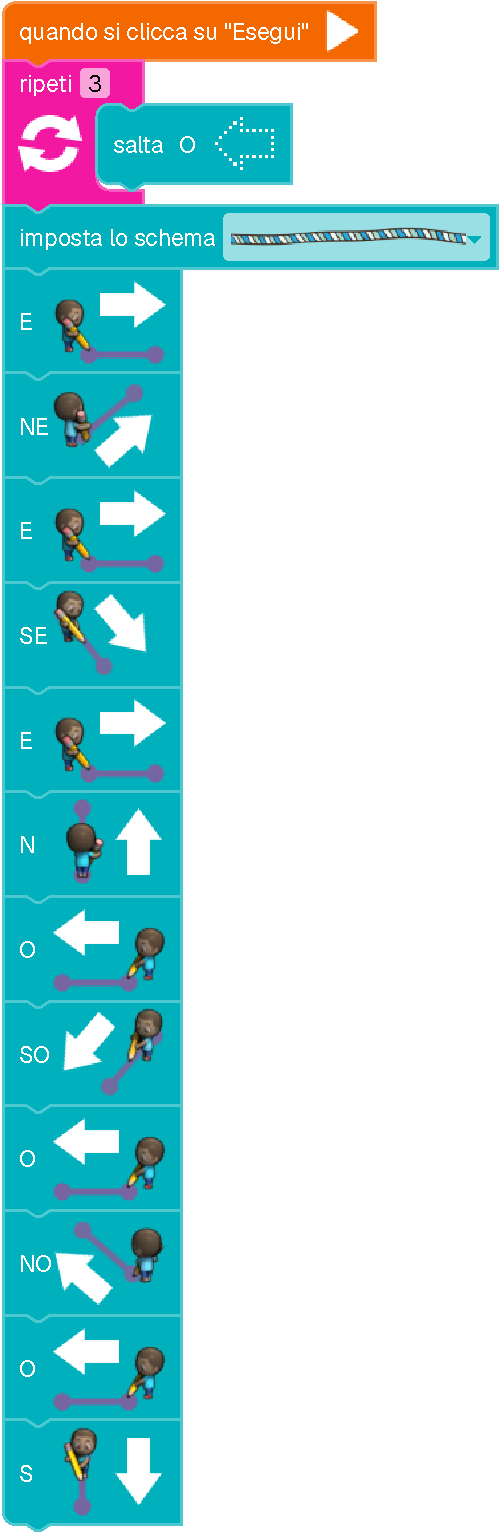
\includegraphics[scale=0.5]{img/codeorg-svg-cap07/pdf/codeorg-trama-ripetuta-programma.pdf}\label{credito:codeorg-artista-trama-programma-1}
\end{minipage}
\end{center}


\section{Attività 4: Labirinti (corso C)}

\ruoliattivita{\ruoloProgrammatore}

Le Lezioni 3, 4, 5, 8, 9 del Corso C sono tutte collocate nell'ambiente ``Labirinti''. L'ambiente è del tutto analogo a quelli dei Corsi A e B, ma, da questo corso in poi, i movimenti del personaggio saranno descritti rispetto a un sistema di riferimento soggettivo centrato sul personaggio, così come abbiamo visto nelle attività unplugged con riferimenti soggettivi (vedere Capitolo~\ref{capitolo-4-movimenti-su-una-griglia} - Movimenti sulla griglia).

Quindi, in questa attività, chi programma vive la scena dal punto di vista del personaggio: quando c'è un'istruzione di movimento, è sempre ``rispetto a dove sta guardando il personaggio''. Se dici al personaggio ``vai avanti'', lui cammina nella direzione in cui è rivolto il suo sguardo.




\section{Altre attività }\label{altre-attivituxe0}

\ruoliattivita{\ruoloProgrammatore}

\subsection{Eventi (corsi A, B, C) }\label{eventi-corsi-a-b-c}

Nella Lezione 12 del Corso A e del Corso B, e nelle lezioni 12, 13 e 16 del Corso C è possibile costruire videogiochi, storie e animazioni facendo parlare personaggi, facendoli muovere e facendoli reagire ad eventi (es. click del mouse, pressione dei tasti freccia sulla tastiera).

Lascia che studenti e studentesse sperimentino con questi livelli. L'introduzione alla creazione di giochi, storie, animazioni è la parte centrale di Scratch, che verrà introdotto nel prossimo capitolo.

\subsection{Artista (corso C) }\label{artista-corso-c}

Nel Corso C, anche nei livelli dedicati all'artista i movimenti vengono espressi rispetto a un sistema di riferimento soggettivo, centrato sull'Artista, ed è presente anche la possibilità di orientarlo di un certo angolo. Puoi lasciare che i tuoi studenti sperimentino intuitivamente e poi, al momento opportuno, collegare quanto emerso dalle loro esplorazioni ai concetti geometrici più formali.


\subsubsection{Lunghezze e angoli nell'Artista}

\ruoliattivita{\ruoloProgrammatore\quad\ruoloEsecutore}

Nell'Artista del Corso C puoi rendere concreto il significato dei numeri presenti nei blocchi.

\begin{center}
\manualeimpostazioni
\begin{tabular}{|K{\dimexpr0.50\linewidth-2\tabcolsep-3\arrayrulewidth/2\relax}|J{\dimexpr0.50\linewidth-2\tabcolsep-3\arrayrulewidth/2\relax}|}
\arrayrulecolor{guideManualeBordo}
\hline
\manualetitolo{2}{ARTISTA CORSO C}
\manualeintestazione
\manualeimmagini{
\includegraphics[scale=0.9]{img/codeorg-svg-cap07/pdf/codeorg-bozza-artista-avanti100.pdf}\label{credito:codeorg-artista-comandi-angoli-1}}
& Fa avanzare l'artista nella direzione in cui guarda e traccia un tratto rettilineo lungo 100 pixel. Il pixel, già incontrato parlando di immagini digitali (vedi~\ref{rappresentare-colori-immagini-video}), viene qui usato come unità per esprimere la lunghezza sullo schermo. \\
\hline
\manualeimmagini{
\includegraphics[scale=0.9]{img/codeorg-svg-cap07/pdf/codeorg-bozza-artista-destra90.pdf}\label{credito:codeorg-artista-comandi-angoli-2}}
& Fa ruotare l'artista su se stesso di 90° verso destra e senza tracciare un nuovo tratto rettilineo. \\
\hline
\end{tabular}
\manualeripristinacolore
\end{center}

Ad esempio, si può proporre di cambiare l'ampiezza in gradi dell'angolo di rotazione impostando valori come 45, 60, 90 o 120 gradi (o cambiando il verso) e poi confrontare la direzione finale con quella iniziale. È importante notare che il valore numerico nel blocco indica l'ampiezza dell'angolo di rotazione rispetto alla direzione attuale dell'artista (quindi non, ad esempio, l'angolo interno della figura che si sta disegnando). Prima di eseguire il programma, può essere utile chiedere di indicare con la mano da quale parte sarà rivolto l'artista per poi confrontare la previsione con il risultato.




\begin{center}
\begin{minipage}{0.94\linewidth}
\centering
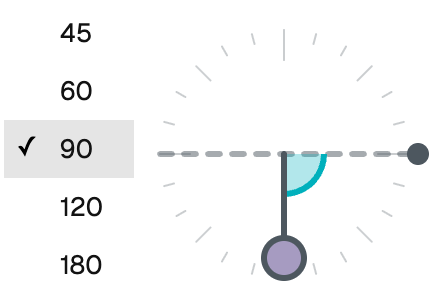
\includegraphics[width=4.2cm]{img/codeorg-artista-schermate/menu-angoli.png}\label{credito:codeorg-artista-selettore-angoli-1}
\par\smallskip
\textbf{Scegliere l'angolo di rotazione}\par
\end{minipage}
\end{center}

\begin{center}
\begin{minipage}{0.94\linewidth}
\centering
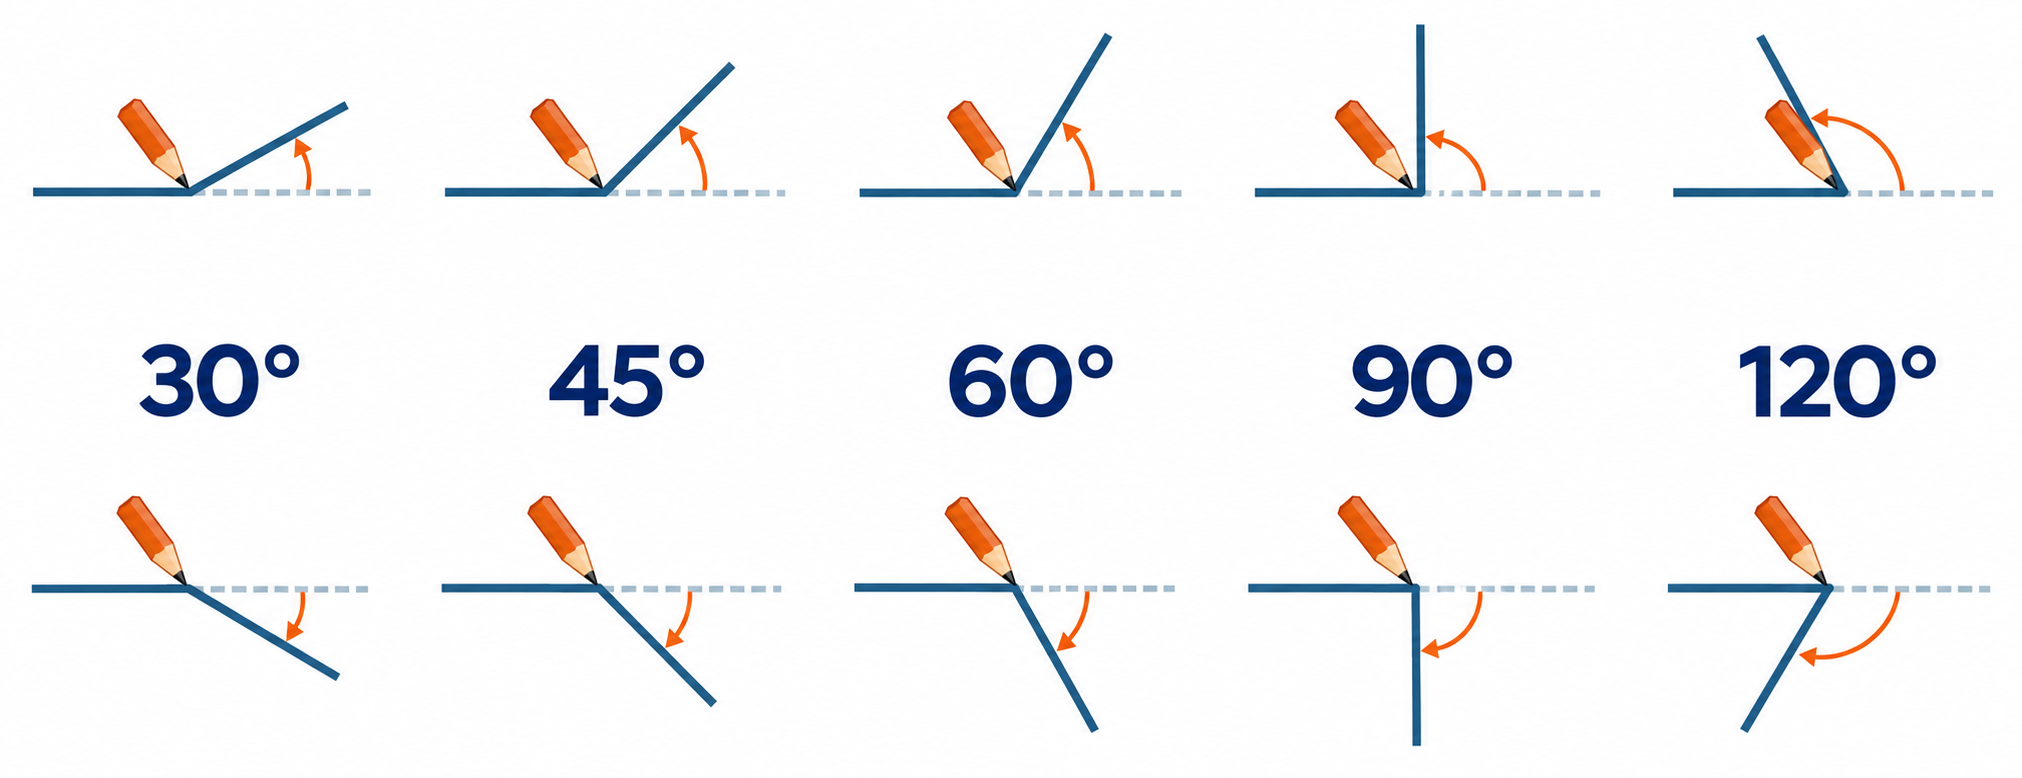
\includegraphics[width=\linewidth]{img/rotazioni-matita.png}\label{credito:rotazioni-matita-1}
\par\smallskip
\textbf{Confrontare le rotazioni.} Da una stessa direzione iniziale, gli esempi mostrano rotazioni di 30, 45, 60, 90 e 120 gradi verso sinistra (sopra) e verso destra (sotto). La linea tratteggiata prolunga la direzione precedente.\par
\end{minipage}
\end{center}

Combinando segmenti e rotazioni si possono costruire anche figure riconoscibili, come questo gattino. Puoi usarlo come spunto per chiedere di individuare le parti del disegno e immaginare quali movimenti permettano di realizzarle; lascia poi che ciascuno inventi una propria figura.

\begin{center}
\begin{minipage}{0.94\linewidth}
\centering
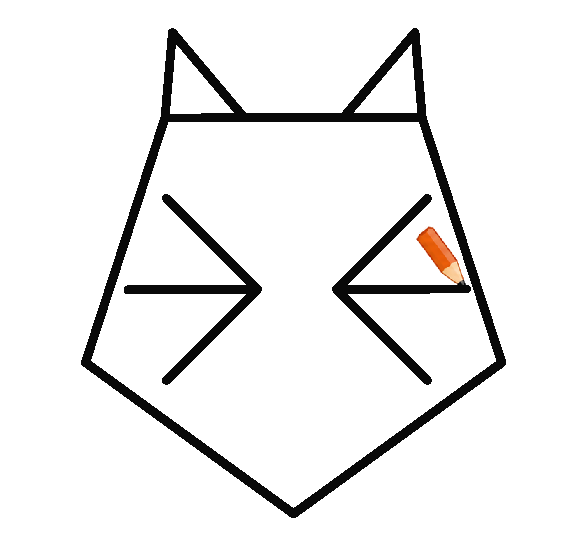
\includegraphics[width=5.2cm]{img/gattino-matita/gattino.pdf}\label{credito:gattino-matita-1}
\end{minipage}
\end{center}

Per continuare a disegnare senza un compito preassegnato, puoi aprire il \textbf{laboratorio libero dell'Artista}: \linkbreve{artista}. È l'ambiente con lunghezze e angoli nei blocchi, distinto dal Laboratorio Artista pre-scolare già usato per i corsi A e B.

\subsection{L'Ora dell'InformaticA (l'Ora del Codice) }\label{lora-dellinformatica-lora-del-codice}

Code.org è diventata famosa per l'iniziativa ``L'ora del Codice'', dal 2025 rinominata ``L'ora dell'InformaticA'' (per maggiormente rimarcare da un lato l'aspetto disciplinare, e dall'altro l'introduzione di elementi di Intelligenza Artificiale). Si tratta di un'iniziativa in cui, più o meno nello stesso periodo (es. la ``Settimana Internazionale dell'Insegnamento dell'Informatica'', che solitamente cade a dicembre - \urloriginale{https://www.csedweek.org/}), le bambine e i bambini di tutto il mondo svolgono almeno un'ora di introduzione alla programmazione. Puoi consultare le attività proposte sul sito: \linkbreve{oraInformaticA}.

\section{Modalità di lavoro }\label{modalituxe0-di-lavoro-4}

L'approccio guidato dalla piattaforma dovrebbe permettervi di far sì che, una volta avviata l'attività, studenti e studentesse procedano in modo autonomo e ciascuno al proprio ritmo. Tuttavia, è importante facilitare e vigilare costantemente sul processo.

\subsection{Debugging }\label{debugging}

Le attività proposte in questo capitolo della guida offrono un contesto autentico per sperimentare la pratica del debugging. Infatti, se escludiamo le attività con i robot educativi, questa è probabilmente la prima volta che gli studenti hanno a che fare realmente con un esecutore automatico, ``meccanico''.

Come abbiamo visto, in informatica, più che applicare una procedura già nota, si tratta spesso di progettarne una che risolva il problema in questione, ma non sia già conosciuta e che, idealmente, possa funzionare anche per altri casi simili appartenenti alla stessa classe di problemi. Sarà quindi normale procedere, almeno in parte, con prove ed errori. Se da un lato all'inizio può essere frustrante vedere che il programma non fa ciò che ci si aspetta, dall'altro--una volta convinti studenti e studentesse che il computer esegue sempre e solo la sequenza di istruzioni che gli vengono date, e in modo sempre ``prevedibile'' e ``ripetibile''--si può accettare più serenamente che l'errore è dovuto a un programma che va rivisto e migliorato perché non aderente agli obiettivi.

Per abituare studenti e studentesse a riconoscere le cause degli errori e correggerli, può essere utile aiutarli a strutturare le fasi di debug, ad esempio proponendo di seguire le fasi spiegate nel box che segue.

\subsubsection{Fasi di debugging}

\begin{enumerate}
\def\labelenumi{\arabic{enumi}.}
\item
  Assicurarsi di aver capito qual è l'obiettivo del protagonista.
\item
  Eseguire il programma: cosa c'è di sbagliato nel comportamento del protagonista?
\item
  Cercare di determinare quali blocchi sono responsabili del comportamento sbagliato (per capirlo meglio può essere utile usare ``Fai un passo'' per eseguire un'istruzione alla volta, vedendo che effetto ha sul programma; oppure far disegnare l'Artista più lentamente).
\item
  Modificare il programma (aggiungere o togliere istruzioni, o modificare i numeri presenti in esse) e poi rieseguirlo.
\item
  Se ancora non funziona, valutare se con le modifiche fatte ci si sta avvicinando all'obiettivo oppure se è meglio annullarle.
\item
  Ritornare al passo 3 fino a che non si è raggiunto l'obiettivo.
\end{enumerate}

\subsection{Programmazione in coppia }\label{programmazione-in-coppia}

Un altro modo di fare debugging è raccontare a un compagno o una compagna che cosa fa il proprio programma. Spesso il solo fatto di spiegare ad alta voce le istruzioni del proprio programma fa capire a chi l'ha creato dove ha sbagliato. Nell'industria informatica, questa pratica è stata istituzionalizzata come metodologia chiamata ``pair programming'', cioè ``programmazione in coppia'' - due programmatori programmano insieme su un solo computer. È una metodologia estremamente utile anche a scuola.

Nella programmazione in coppia, pensiamo la coppia come a un equipaggio da rally: da una parte c'è il \textbf{pilota}, dall'altra il \textbf{navigatore}. Come in un vero rally, il pilota ha in mano il ``volante'', cioè il mouse: il pilota materialmente guida il programma, clicca, trascina i blocchi, scrive il codice. Il suo obiettivo è arrivare a un programma funzionante, proprio come il pilota vuole portare l'auto al traguardo. Mentre lavora, però, non lo fa in silenzio: il pilota racconta ad alta voce al navigatore che cosa sta facendo, passo dopo passo, spiegando perché sceglie un certo blocco o lo mette in un certo punto. Il compagno o la compagna con il ruolo di navigatore potrà dare dei suggerimenti ma alla fine sarà il pilota a prendere le decisioni finali: ha il volante/mouse in mano.

Il navigatore, invece, è come il copilota nel rally: osserva con attenzione ciò che fa il pilota e ascolta ciò che dice, ma non tiene il volante. Il suo compito è guardare bene la ``strada'' che hanno davanti, in questo caso il puzzle di programmazione, e aiutare il pilota a non perdersi. Può notare errori, proporre correzioni, suggerire strade alternative: ``E se invece provassimo a mettere questo blocco qui?'', ``Secondo me così il personaggio non arriverà dove vogliamo''. Mentre il pilota si concentra sui dettagli, il navigatore mantiene la visione d'insieme: verifica se il programma sta davvero procedendo nella direzione giusta per risolvere il problema.

Ogni tanto si scambiano i ruoli: chi guidava diventa il navigatore e chi faceva il navigatore passa al volante. All'inizio sarà l'insegnante a guidare questo scambio e a ricordare i compiti di ciascuno, ma l'obiettivo è che studenti e studentesse imparino pian piano a collaborare in modo autonomo.

Come insegnante dovrai fare attenzione nel formare (e, se necessario, separare) le coppie e, soprattutto, nel far rispettare i ruoli: un pilota che non considera il navigatore o un navigatore prepotente sono da evitare!

In questo video viene spiegata la metodologia: \linkbreve{coppia}.

Su Code.org è possibile cliccare sulla casella accanto alla scritta ``Sto lavorando in coppia'' che appare una volta effettuato il login, quindi cliccare prima sul nome del compagno o della compagna con cui si sta lavorando e poi sul pulsante ``Aggiungi partner'', per essere sicuri che vengano tracciati i progressi di entrambi i membri della coppia (o anche di gruppi più numerosi).

\subsection{Evitare l'effetto ``basta superare il livello'' }\label{evitare-leffetto-basta-superare-il-livello}

La modalità con cui progrediscono le lezioni di Code.org (piccoli puzzle da superare) dovrebbe essere congeniale perché studenti e studentesse li considereranno livelli da superare in un videogioco. Tuttavia, è importante evitare che questo generi l'idea che basti ``far venire gli esercizi'' (senza aver capito perché la soluzione proposta è corretta, oppure proponendo soluzioni molto lunghe e ripetitive da scrivere), magari addirittura gareggiando per chi li completa prima. Di seguito discutiamo alcune strategie per superare questo approccio ingenuo.


\subsection{Esistono più programmi corretti!}


Uno degli aspetti più belli dell'informatica è che lo stesso problema può avere molte soluzioni diverse, tutte valide. In Code.org, questo diventa subito evidente: programmi differenti possono portare il personaggio allo stesso obiettivo, pur utilizzando blocchi o strategie non identiche. È importante valorizzare questo aspetto: non si tratta di trovare ``la'' risposta giusta, ma di scoprire che esistono modi diversi per arrivare allo stesso risultato! Questa varietà permette attività ricchissime in classe:

\begin{itemize}
\item
  confrontare soluzioni diverse;
\item
  raccontare come ciascuno ha ragionato;
\item
  osservare cosa cambia se si sposta un blocco;
\item
  scoprire nuove idee guardando il lavoro degli altri.
\end{itemize}

In questo modo la programmazione diventa un terreno di dialogo e creatività: ogni soluzione è un punto di vista, e il confronto tra programmi aiuta a capire meglio sia il problema sia i concetti informatici in gioco.

\subsection{La sfida è usare meno blocchi possibile }\label{la-sfida-uxe8-usare-meno-blocchi-possibile}

Nell'Area di lavoro viene sempre indicato il numero di blocchi attualmente utilizzati nel programma. Solitamente, se si risolve un puzzle usando un numero elevato di blocchi, Code.org suggerisce che sarebbe stato possibile farlo con meno. È importante che, piano piano, studenti e studentesse comincino ad apprezzare programmi che fanno uso di meno blocchi, in quanto più chiari e semplici da comprendere (e anche da realizzare, ad esempio, senza dover trascinare lunghe sequenze di blocchi tutti uguali). Dunque, è importante suggerire di non superare il numero di blocchi indicato come obiettivo nel titolo dell'Area di lavoro.

L'esempio del blocco Ripeti è lampante: non è necessario per risolvere i semplici problemi proposti in questi corsi, ma consente di realizzare programmi decisamente più brevi (cioè con meno blocchi) e quindi più leggibili.

\begin{center}
\begingroup
\setlength{\tabcolsep}{5pt}
\setlength{\arrayrulewidth}{0.4pt}
\arrayrulecolor{black!40}
\renewcommand{\arraystretch}{1.15}
\begin{tabular}{|c|c|c|}
\hline
\begin{minipage}[c]{\dimexpr0.30\linewidth-2\tabcolsep-4\arrayrulewidth/3\relax}\centering\vspace{5pt}
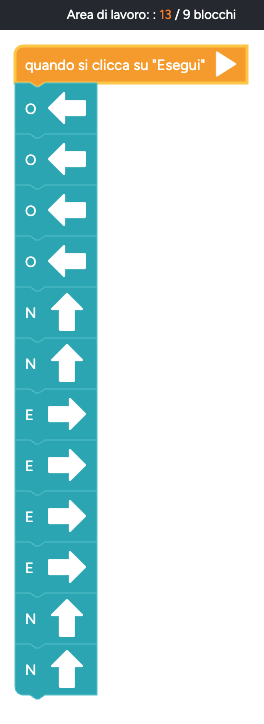
\includegraphics[width=0.988764\linewidth]{img/codeorg-confronto-blocchi/programma-13.png}\label{credito:codeorg-confronto-13-9-1}\par\vspace{5pt}
\end{minipage}
& \begin{minipage}[c]{\dimexpr0.40\linewidth-2\tabcolsep-4\arrayrulewidth/3\relax}\raggedright
Ad esempio, il programma di sinistra usa 13 blocchi ma se ne poteva realizzare un altro con lo stesso effetto usando solo 9 blocchi (immagine a destra)!
\end{minipage}
& \begin{minipage}[c]{\dimexpr0.30\linewidth-2\tabcolsep-4\arrayrulewidth/3\relax}\centering\vspace{5pt}
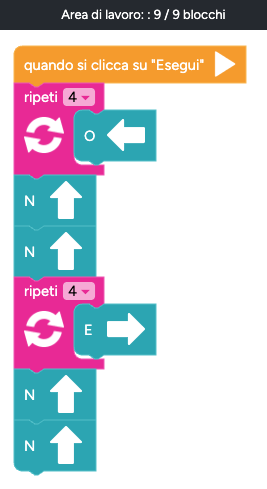
\includegraphics[width=\linewidth]{img/codeorg-confronto-blocchi/programma-9.png}\label{credito:codeorg-confronto-13-9-2}\par\vspace{5pt}
\end{minipage} \\
\hline
\end{tabular}
\endgroup
\end{center}

\bigskip

A volte compare un numero rosso che indica il numero massimo di volte in cui si può usare un blocco nel programma.


\begin{center}

\includegraphics[width=2.8cm]{img/codeorg-confronto-blocchi/codeorg-est-limite-1.pdf}\label{credito:codeorg-est-limite-1}
\end{center}


Questo è un altro modo su Code.org per ``forzare'' alunne e alunni a utilizzare, ad esempio, il blocco Ripeti.

\section{Valore costruzionista }\label{valore-costruzionista-4}

Da un punto di vista metodologico, in Code.org la scoperta di nuovi concetti è inizialmente molto vincolata da un elevato scaffolding, cioè un insieme di \emph{sostegni temporanei} che aiutano bambini e bambine a procedere passo passo fino a diventare autonomi. Pian piano viene concessa loro maggiore libertà creativa \parencite{resnick-rusk-2020}. Tuttavia, in ogni puzzle da risolvere viene spesso richiesto di usare nuovi blocchi lasciando a studenti e studentesse la possibilità di esplorarne il funzionamento per capire come utilizzarli per raggiungere gli obiettivi e superare i livelli.

Per poter aumentare la libertà di esplorazione anche quando si programma su Code.org è nato, in direzione costruzionista, l'approccio metodologico chiamato \emph{Usa-Modifica-Crea}, che descriviamo di seguito.

\subsection{Usa, Modifica, Crea }\label{usa-modifica-crea}

In questo approccio metodologico (o meglio, famiglia di approcci metodologici - poiché è stato declinato in molti modi diversi), studenti e studentesse imparano usando programmi già scritti, modificandoli e, infine, creando programmi tutti loro.

Le attività sono solitamente organizzate in tre fasi. Le fasi hanno un ordine logico, ma non sono rigide: si può andare avanti o indietro più volte.

Le descriviamo di seguito, affidandoci a \AtNextCite{\defcounter{maxnames}{99}}\textcite{caserio-etal-umc}.

\begin{enumerate}
\item
  Fase ``\textbf{Usa}'': ``Provo il programma degli altri''

In questa prima fase si esegue un programma già pronto, costruito dall'insegnante o da altri, rispondendo poi a domande di riflessione.


\begin{itemize}
\item
  Il programma non è banale: deve essere un po' ``curioso'' o ``bello da vedere'' (es. un minigioco o una storia autoconclusiva) e, idealmente, contenere i nuovi concetti che si vogliono introdurre.
\item
  Bambini e bambine eseguono il programma senza vedere le istruzioni di cui è composto: osservano semplicemente ciò che succede sullo schermo, e rispondono a domande di riflessione su ciò che hanno esperito. In questo modo studenti e studentesse si concentrano prima sul descrivere e interpretare il comportamento del programma e non sulle istruzioni.
\end{itemize}

\item
  Fase ``\textbf{Modifica}'': ``Metto mano al codice''

Nella seconda fase, studenti e studentesse possono vedere le istruzioni che costituiscono il programma. L'obiettivo è leggere le istruzioni (i blocchi), esplorarli e collegarli a ciò che accade sullo schermo quando il programma viene eseguito. L'insegnante in questa fase può proporre vari tipi di attività, quali:

\begin{itemize}
\item
  Richiedere di apportare modifiche alle istruzioni del programma, come ad esempio spostare o sostituire un blocco, o cambiare un numero dentro a un blocco. Studenti e studentesse eseguiranno quindi di nuovo il programma osservando che cosa è cambiato nell'effetto.
\item
  Richiedere di fare previsioni. Prima di apportare la modifica, l'insegnante invita studenti e studentesse a formulare esplicitamente un'ipotesi sull'effetto che avrà la modifica sul risultato dell'esecuzione del programma. Solo dopo che ciascuno avrà formulato la propria previsione si potrà procedere con la modifica del programma, confrontando le varie ipotesi con il risultato.
\item
  Richiedere di apportare modifiche alle istruzioni del programma con un obiettivo dato. Viene dato un obiettivo esplicito e circoscritto, per esempio: cambiare un dettaglio grafico; variare in piccola parte il funzionamento del programma. Studenti e studentesse quindi proveranno, sbaglieranno, ritenteranno finché non raggiungono il risultato richiesto.
\end{itemize}


In questa fase si lavora molto sulla curiosità e sulla sperimentazione, orientando sempre le attività di modifica a comprendere meglio i nuovi concetti da introdurre.


\item
  Fase ``\textbf{Crea}'': ``Costruisco il mio programma''


Nella terza fase, studenti e studentesse sono invitati a creare un proprio programma personale, utilizzando anche i nuovi concetti appresi. La creazione può essere più o meno dirompente rispetto ai progetti delle fasi precedenti.


\begin{itemize}
\item
  Creazione come evoluzione delle modifiche. Studenti e studentesse partono dal programma proposto dall'insegnante, ma decidono di modificare in modo più profondo la grafica o il funzionamento. Il tuo ruolo di insegnante in questo caso sarà quello di controllare che, nelle loro creazioni, studenti e studentesse utilizzino i nuovi concetti introdotti.
\item
  Creazione libera con alcuni vincoli. Studenti e studentesse possono progettare un programma anche molto diverso da quelli visti prima, ma con qualche vincolo chiaro, ad esempio: usare alcuni blocchi obbligatori; rispettare un certo comportamento generale dei personaggi.
\end{itemize}

\end{enumerate}

In questo modo, anche nella creazione più libera, bambini e bambine devono comunque mettere in gioco i nuovi concetti, consolidandoli attraverso le proprie idee.


\textbf{Un esempio di materiale didattico completo} (che comprende sia le schede studenti che una guida passo-passo per l'insegnante) per introdurre il concetto di ciclo utilizzando l'Artista di Code.org in una classe di terza primaria è disponibile all'indirizzo: \urloriginale{https://lodi.ml/umc}.

\section{Aspetti informatici }\label{aspetti-informatici-3}

In queste attività studenti e studentesse incontrano per la prima volta un vero linguaggio di programmazione. È fatto di blocchetti colorati, ma ha tutte le caratteristiche di un linguaggio formale: ad esempio, ha una sintassi (i blocchetti si incastrano solo in un certo modo) e una semantica (es. la sequenza di istruzioni incluse nella forma a C di un Ripeti viene eseguita il numero di volte indicato nel blocco stesso).

In queste attività studenti e studentesse non si limitano a ``giocare con i blocchi'', ma incontrano alcune idee chiave di informatica.

\begin{itemize}
\item
  \textbf{Algoritmo vs programma}. I puzzle dei Labirinti e dell'Artista rendono visibile il passaggio dall'algoritmo (la sequenza di istruzioni pensata a voce o su carta) al programma (cioè l'algoritmo tradotto in un linguaggio di programmazione eseguibile dal computer). La stessa strategia usata negli esercizi unplugged (sequenze di frecce o istruzioni) deve ora essere tradotta in blocchi, rispettando la sintassi del linguaggio.
\item
  \textbf{Sequenza e ciclo come prime strutture di controllo}. La maggior parte dei puzzle può essere risolta con semplici sequenze; l'introduzione del blocco Ripeti permette di ``compattare'' programmi lunghi e ripetitivi, facendo emergere l'idea che un buon programma non è solo quello che ``funziona'', ma anche quello più leggibile e manutenibile (quindi ad esempio ha meno blocchi ed è più chiaro).
\item
  \textbf{Parametri e generalizzazione}. Nei livelli dell'Artista, trovi alcuni blocchi che richiedono di specificare dei numeri. In informatica, questi numeri sono chiamati parametri: indicano quanto deve muoversi o ruotare l'Artista. Cambiando il parametro, puoi ottenere disegni diversi: non stai più programmando ``questo quadrato preciso'', ma stai programmando ``un quadrato di lato di lunghezza x'', semplicemente modificando il numero. È una prima forma di generalizzazione, perché studenti e studentesse capiscono che un programma può funzionare anche quando cambiano i valori.
\item
  \textbf{Esecutore meccanico}. Il personaggio sullo schermo si comporta come un esecutore ``ottuso'': fa esattamente ciò che c'è scritto nel programma, né più né meno. Insistere su questo aspetto aiuta studenti e studentesse a costruirsi una prima immagine mentale del calcolatore come sistema deterministico che esegue alla lettera una sequenza di istruzioni.
\item
  \textbf{Previsione, esecuzione e debugging.} In questo capitolo, nella sezione relativa alla Modalità di lavoro, il debugging è già stato presentato come pratica centrale per accogliere e affrontare gli errori in modo sereno e sistematico. In questo modo studenti e studentesse imparano che l'errore non è un fallimento, ma un'informazione preziosa sul funzionamento del proprio programma.
\end{itemize}

\section{Relazione con l'informatica nelle Indicazioni Nazionali 2025 }\label{relazione-con-linformatica-nelle-indicazioni-nazionali-4}

Relativamente alle Indicazioni Nazionali 2025, queste attività contribuiscono allo sviluppo delle seguenti competenze, obiettivi e conoscenze (queste ultime inserite nelle Indicazioni Nazionali 2025 a titolo di esempio, non prescrittive).


\subsubsection{Competenze (alla fine della scuola primaria) nella disciplina Matematica}


\begin{itemize}
\item
  \emph{Scrivere e comprendere semplici programmi, espressi in elementari linguaggi di programmazione a scopo didattico, e valutarne l'adeguatezza rispetto al compito che si vuole automatizzare.}
\end{itemize}



\subsubsection{Obiettivi (alla fine della terza primaria) nella disciplina Matematica}


\begin{itemize}
\item
  \emph{Scrivere semplici programmi e verificare, mediante la loro esecuzione, se svolgono il compito previsto ed eventualmente correggerli.}
\end{itemize}


\subsubsection{Obiettivi (alla fine della terza primaria) nella disciplina Tecnologia}


\begin{itemize}
\item
  \emph{Creare, selezionare e usare semplici testi o disegni, usando strumenti informatici.}
\end{itemize}

\subsubsection{Conoscenze (scuola primaria) nella disciplina Matematica}

\begin{itemize}
\item
  \emph{Concetto di algoritmo e sua esecuzione rigorosa.} In particolare qui si lavora sulla creazione ed esecuzione di programmi, cioè algoritmi scritti in un linguaggio di programmazione (qui, in particolare, il linguaggio a blocchi di Code.org).
\item
  \emph{Strutture di controllo fondamentali di un linguaggio di programmazione e reazione agli eventi.}
\item
  \emph{Controllo di correttezza dei programmi.}
\end{itemize}

\section{Suggerimenti per ulteriori attività}\label{suggerimenti-per-ulteriori-attivituxe0-e-riferimenti-4}

\printbibliography[heading=none,keyword={cap7},category={attivita}]

\begin{rimandiquaderno}
Se possiedi il volume studente \emph{Sulle orme di Milù -- Informatica}
(Mondadori Education, 2026), puoi usare i rimandi seguenti per affiancarlo
alle attività di questo capitolo.\par\smallskip

\begin{itemize}[leftmargin=*,itemsep=5pt,topsep=4pt]
\item \textbf{Introduzione a Code.org (Attività 1).} Alle pagg.~28--29, le schede BENVENUTI IN CODE.ORG accompagnano i primi passi negli ambienti guidati dei corsi di Introduzione all'Informatica.
\item \textbf{Labirinti (Attività 2).} Le schede LABIRINTI~\textbullet{}~2 (pagg.~30--31) si collegano alle lezioni nell'ambiente Labirinti dei corsi A e B e comprendono una guida sintetica all'effetto dei blocchi-direzione. Se mancano computer o tablet, oppure per assegnare un compito unplugged, la scheda IL VIAGGIO DEL POLPO (pag.~31) propone su carta lo stesso esercizio online: l'ambientazione cambia, ma le soluzioni restano le stesse. \textbf{Soluzione:} N, E, E, E, S. \textbf{Sfida finale con soli 4 blocchi:} N, ripeti 3 volte [E], S. Un'attività identica, con solo ambientazione diversa, online, è disponibile a  \linkbreve{codeLabirinto}. (NB: il blocco “quando si clicca su “Esegui”” non è presente né conteggiato nel
Quaderno di Informatica, mentre è conteggiato su Code.org).
\item \textbf{Artista (Attività 3).} Le schede ARTISTA (pagg.~32--33) corrispondono alle attività nell'ambiente Artista dei corsi A e B; a pag.~32 è presente anche una guida sintetica all'effetto dei blocchi.
\item \textbf{Labirinti (Attività 4).} Le schede LABIRINTI~\textbullet{}~3 (pagg.~34--35) si collegano alle lezioni nell'ambiente Labirinti del Corso C e comprendono una guida sintetica ai blocchi di movimento e rotazione. Se mancano computer o tablet, oppure per assegnare un compito unplugged, usare l'esercizio di pag.~35. \textbf{Soluzione con 8 blocchi:} avanti, destra, avanti, avanti, avanti, avanti, destra, avanti. \textbf{Sfida finale con soli 6 blocchi:} avanti, destra, ripeti 4 volte [avanti], destra, avanti. Lo stesso percorso, con un'ambientazione diversa, è disponibile online a \linkbreve{codeRapido}. (NB: il blocco “quando si clicca su “Esegui”” non è presente né conteggiato nel
Quaderno di Informatica, mentre è conteggiato su Code.org).
\end{itemize}
\end{rimandiquaderno}

\section{Riferimenti}\label{riferimenti-cap7}

\printbibliography[heading=none,keyword={cap7},notcategory={attivita}]
